\documentclass[10pt]{beamer}
% \documentclass[handout,10pt]{beamer}
\usepackage{my_style}

%%%%%%%%%%%%%%%%%%%%%%%%%%%%%%%%%%%%%%%%%%%%%%%%%%%%%%%%%%%%%%%%%%%%%%%%
%%%%%%%%%%%%%%%%%%%%%%%%%%%%%%%%%%%%%%%%%%%%%%%%%%%%%%%%%%%%%%%%%%%%%%%%

\title[Math/CS 375]{Lecture 13 - B}
\subtitle{\S 8.2, 8.3 Markov Chains}


\begin{document}
% -------------------------------------------------
\begin{frame}
  \titlepage
\end{frame}

%%%%%%%%%%%%%%%%%%%%%%%%%%%%%%%%%%%%%%%%%%%
\begin{frame}{Goals}
We will answer these questions:\\[3mm]
\begin{itemize}
    \item What is a Markov chain?
    \item How do transition matrices model state evolution?
    \item Why do Markov chains always have a special eigenvalue?
    \item How do eigenvectors describe long-term behavior?
\end{itemize}
\end{frame}

%%%%%%%%%%%%%%%%%%%%%%%%%%%%%%%%%%%%%%%%%%%%%%%%%%%%%%%%%%%%%%%%%%%%%%%%
\sectionframe{Markov Chains}
%%%%%%%%%%%%%%%%%%%%%%%%%%%%%%%%%%%%%%%%%%%%%%%%%%%%%%%%%%%%%%%%%%%%%%%%


\begin{frame}{Markov Chains}
\define{Markov Chain}{
\begin{itemize}
    \item A \textbf{Markov Chain} models how a system randomly transitions between a finite set of states.
    \item The probability of the next state depends only on the current state (not the past).
\end{itemize}
}

\begin{itemize}
    \item States are denoted by integers $\{1,2,\ldots,n\}$
    \item Probability of jumping from state $j$ to state $i$ is $P_{ij}$
\end{itemize}

\vspace{5mm}
\textbf{Example:} Weather Prediction
\begin{itemize}
    \item \textbf{System}: Weather conditions observed every 24 hours
    \item \textbf{States}: $\{$1=Sunny, 2=Cloudy, 3=Rainy$\}$
    \item \textbf{Probability}: $P_{32}=0.3 \implies$  $30\%$ chance of rain if today is cloudy
\end{itemize}
\end{frame}

%%%%%%%%%%%%%%%%%%%%%%%%%%%%%%%%%%%%%%%%%%%%%%%%%%%%%%%%%%%%%%%%%%%%%%%%

\begin{frame}{Transition Diagram}

\vspace{4mm}

\begin{center}
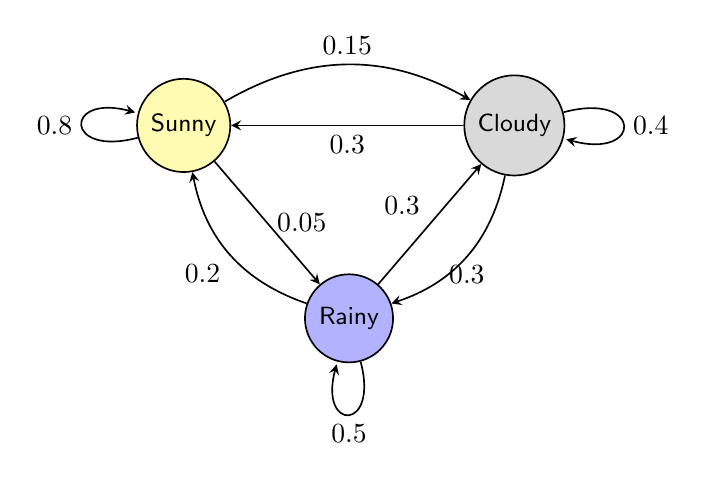
\begin{tikzpicture}[>=stealth, auto, node distance=3cm, semithick,scale=0.7]
    % Define styles for states
    \tikzstyle{state}=[circle, draw, minimum size=1cm, font=\sffamily\small]

    % Nodes with color fill
    \node[state, fill=yellow!30] (Sunny) at (-3,1.5) {Sunny};
    \node[state, fill=gray!30] (Cloudy) at (3,1.5) {Cloudy};
    \node[state, fill=blue!30] (Rainy) at (0,-2) {Rainy};

    % Edges with arrows and transition probabilities
    \path
        (Sunny) edge [->, loop left] node {0.8} ()
               edge [->, bend left] node {0.15} (Cloudy)
               edge [->,right] node {0.05} (Rainy)
        (Cloudy) edge [->, below] node {0.3} (Sunny)
                edge [->, loop right] node {0.4} ()
                edge [->, bend left] node [below] {0.3} (Rainy)
        (Rainy) edge [->, bend left] node {0.2} (Sunny)
               edge [->] node {0.3} (Cloudy)
               edge [->, loop below] node {0.5} ();
\end{tikzpicture}\\
\begin{itemize}
    \item Vertices (Sunny, Cloudy, Rainy) represent states
    \item Number on the arrows represent chance of switching between states
    \item Example: If today is Sunny, tomorrow will be sunny with an $80\%$ chance
\end{itemize}
\end{center}
\end{frame}


%%%%%%%%%%%%%%%%%%%%%%%%%%%%%%%%%%%%%%%%%%%%%%%%%%%%%%%%%%%%%%%%%%%%%%%%
\begin{frame}[fragile]{Transition Matrix}
\cols{\begin{center}
    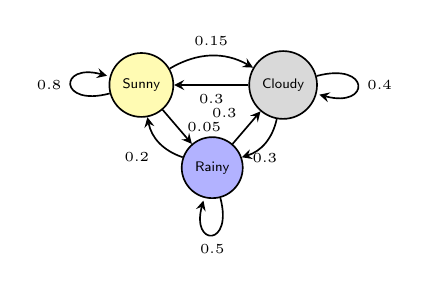
\begin{tikzpicture}[>=stealth, auto, node distance=3cm, semithick,scale=0.3]
        % Define styles for states
        \tikzstyle{state}=[circle, draw, minimum size=0.5cm, font=\sffamily\tiny]
    
        % Nodes with color fill
        \node[state, fill=yellow!30] (Sunny) at (-3,1.5) {Sunny};
        \node[state, fill=gray!30] (Cloudy) at (3,1.5) {Cloudy};
        \node[state, fill=blue!30] (Rainy) at (0,-2) {Rainy};

    % Edges with arrows and transition probabilities
    \path
        (Sunny) edge [->, loop left] node {\tiny 0.8} ()
               edge [->, bend left] node {\tiny 0.15} (Cloudy)
               edge [->,right] node {\tiny 0.05} (Rainy)
        (Cloudy) edge [->, below] node {\tiny 0.3} (Sunny)
                edge [->, loop right] node {\tiny 0.4} ()
                edge [->, bend left] node [below] {\tiny 0.3} (Rainy)
        (Rainy) edge [->, bend left] node {\tiny 0.2} (Sunny)
               edge [->] node {\tiny 0.3} (Cloudy)
               edge [->, loop below] node {\tiny 0.5} ();
    \end{tikzpicture}
    \textbf{Transition Diagram}
    \end{center}
}{   
\begin{center}
    
$$P =
\left(%
\begin{array}{lll}
  .8 & .3 & .2 \\
  .15 & .4 & .3 \\
  .05 & .3 & .5 \\
\end{array}%
\right)
$$
\textbf{Transition Matrix}
\end{center}
}
\vspace{1cm}
\begin{itemize}
    \item Summarize a diagram into a $3\times3$ \textbf{transition matrix} $P$
    \item Element $P_{ij}$ is the probability of going to state $i$ from state $j$. 
    \item The columns of $P$ must add up to 1
\end{itemize}
\end{frame}

%%%%%%%%%%%%%%%%%%%%%%%%%%%%%%%%%%%%%%%%%%%%%%%%%%%%%%%%%%%%%%%%%%%%%%%%

\begin{frame}[fragile]{Transition Matrix}

\[
\begin{tabular}{c l|ccc}
 &  & \multicolumn{3}{c}{\textbf{current}} \\[2pt]
 &  & Sunny & Cloudy & Rainy \\[3mm] \hline
\multirow{3}{*}{\rotatebox{90}{\textbf{future$\quad$}}}
 & Sunny  & 0.8  & 0.3  & 0.2  \\[3mm]
 & Cloudy & 0.15 & 0.4  & 0.3  \\[3mm]
 & Rainy  & 0.05 & 0.3  & 0.5
\end{tabular}
\]
\begin{itemize}
    \item Column represents current state
    \item Row represents future state
    \item $P_{ij}$ represents odds of transitioning to state $i$ from state $j$
    \item $P_{12} = 0.3$ is the chance of  being cloudy tomorrow if today is sunny
\end{itemize}

\end{frame}

%%%%%%%%%%%%%%%%%%%%%%%%%%%%%%%%%%%%%%%%%%%%%%%%%%%%%%%%%%%%%%%%%%%%%%%%

\begin{frame}{Modeling Example}

\begin{example}
On any given day Gary is either cheerful (C), so-so (S), or glum (G). 
\begin{itemize}
    \item If he is cheerful today, then he will be C, S, or G tomorrow with respective probabilities 0.5, 0.4, 0.1. 
    \item If he is feeling so-so today, then he will be C, S, or G tomorrow with probabilities 0.3, 0.4, 0.3. 
    \item If he is glum today, then he will be C, S, or G tomorrow with probabilities 0.2, 0.3, 0.5.
\end{itemize}
\end{example}

\begin{itemize}
    \item System: Gary's mood each day
    \item States: $\{$C,S,G$\}$
    \item Transition Matrix:
    $$
    P = \begin{bmatrix}
        0.5 & 0.3 & 0.2\\
        0.4 & 0.4 & 0.3\\
        0.1 & 0.3 & 0.5
    \end{bmatrix}
    $$
\end{itemize}

\end{frame}

%%%%%%%%%%%%%%%%%%%%%%%%%%%%%%%%%%%%%%%%%%%%%%%%%%%%%%%%%%%%%%%%%%%%%%%%
\sectionframe{Evolution of a Markov Chain}
%%%%%%%%%%%%%%%%%%%%%%%%%%%%%%%%%%%%%%%%%%%%%%%%%%%%%%%%%%%%%%%%%%%%%%%%

\begin{frame}{State Vectors}

\begin{itemize}
    \item We may think of the Markov chain as an \textit{operator} that describes how a \textbf{state vector}  $x_0$ will evolve 
    \vfill

    \item A state vector describes a distribution
    $$x_0=\begin{bmatrix}
        x_{01}\\
        x_{02}\\
        x_{03}
    \end{bmatrix}$$
    where the elements are positive weights satisfying $x_{01}+ x_{02} + x_{03}=1$   
    \vfill

    \item The product 
    $$ x_1 = P x_0$$
    describes the \textbf{new distribution} after one discrete time step
\end{itemize}
    
\end{frame}


\begin{frame}{Exam Grade Example}

    \begin{example}
        \begin{itemize}
            \item If a student gets an A on an exam, the chances are 0.7, 0.2, 0.1 of getting an A, B, or C on the next exam.
            \item If a student gets a $B$, the chances are 0.3, 0.5, 0.2.
            \item If a student gets a $C$, the chances are 0.1, 0.6, 0.3. 
        \end{itemize}
    \end{example}
\begin{itemize}

    \item Suppose half the class gets an A, and half the class gets a C
    $$x_0 = \begin{bmatrix}
        0.5 \\0 \\ 0.5
    \end{bmatrix}$$
    \item On the next exam 
    $$x_1= Px_0=
    \begin{bmatrix}
        0.7 & 0.3 & 0.1\\
        0.2 & 0.5 & 0.6\\
        0.1 & 0.2 & 0.3
    \end{bmatrix}\begin{bmatrix}
        0.5 \\ 0 \\0.5 
    \end{bmatrix} = \begin{bmatrix}
        0.4 \\0.4\\0.2
    \end{bmatrix}
    $$
    $40\%$ will get an A, $40\%$ will get a B, $20\%$ will get a C 
\end{itemize}
\end{frame}

%%%%%%%%%%%%%%%%%%%%%%%%%%%%%%%%%%%%%%%%%%

\begin{frame}{Keep Iterating}

\begin{itemize}
    
    \item After Exam 1:
        $$x_0 = \begin{bmatrix}
        0.5 \\0 \\ 0.5
    \end{bmatrix}$$

    \item After Exam 2:
    $$
    x_1=\begin{bmatrix}
        0.4 \\0.4\\0.2
    \end{bmatrix}
    $$

    \item After Exam 3:
        $$
    x_2=Px_1=\begin{bmatrix}
        0.42 \\0.40\\0.18
    \end{bmatrix}
    $$
    \item After Exam 4:
    $$
    x_3=Px_2=\begin{bmatrix}
        0.432 \\0.392\\0.176
    \end{bmatrix}
    $$
    
\end{itemize}
\end{frame}


%%%%%%%%%%%%%%%%%%%%%%%%%%%%%%%%%%%%%%%%%%

\begin{frame}{One Day vs Many Days}
\begin{itemize}
    \item The transition matrix $P$ describes what happens in \emph{one} time step
    \item What if we want to know what happens after:
    \begin{itemize}
        \item 2 days?
        \item 10 days?
        \item A year?
    \end{itemize}
\end{itemize}

\question{
How do we compute the probability of moving between states over multiple days?
}
\end{frame}

\begin{frame}{Matrix Powers}
\begin{itemize}
    \item If $x_1=Px_0$ then $x_2$ will be given by 
    \begin{align*}
        x_2 = Px_1 \\
        x_2 = P(Px_0)\\
        x_2 = P^2 x_0
    \end{align*}
    \item $P^2$ describes probabilities after two transitions
    \item In general $P^k$ describes probabilities after $k$ transitions
    \item Entry $(i,j)$ of $P^k$ is:
    \[
    P_{ij}^k=\Pr(\text{state } i \text{ after } k \text{ steps} \mid \text{given } \text{state } j \text{ initially})
    \]
\end{itemize}

\keyidea{
Matrix multiplication combines probabilities across time.
}
\end{frame}

\begin{frame}{Example}

\begin{example}
If today is sunny, what is the probability that it will be rainy three days later?   
$$P =
\left(%
\begin{array}{lll}
  .8 & .3 & .2 \\
  .15 & .4 & .3 \\
  .05 & .3 & .5 \\
\end{array}%
\right)
$$
\end{example}

\begin{itemize}
    \item Calculate $P^3=PPP$
    $$
    P^3=\begin{bmatrix}
    0.6365  &  0.4815 &   0.4400\\
    0.2153  &  0.2665 &   0.2775\\
    0.1483  &  0.2520 &   0.2825
    \end{bmatrix} 
    $$
    \item Sunny today $\implies$ column 1
    \item Rainy 3 days from now $\implies $ row 3
    \item The probability of being rainy 3 days if today is sunny is 
    $$P^3_{31} = 0.1483= 14.5\% \text{ chance}$$
\end{itemize}
\end{frame}



%%%%%%%%%%%%%%%%%%%%%%%%%%%%%%%%%%%%%%%%%%%%%%%%%%%%%%%%%%%%%%%%%%%%%%%%
\sectionframe{Absorbing States}
%%%%%%%%%%%%%%%%%%%%%%%%%%%%%%%%%%%%%%%%%%%%%%%%%%%%%%%%%%%%%%%%%%%%%%%%
\begin{frame}[shrink]{Broken Machine Example}{The Setting up the matrix}
\begin{example}
\cols{

    An office printer has three states:  
    \begin{itemize}
        \item State 1: Working 
        \item State 2: Temporarily Broken
        \item State 3: Permanently Broken   
    \end{itemize}
Each day it is in one of these states. Find the transition matrix.
}{
    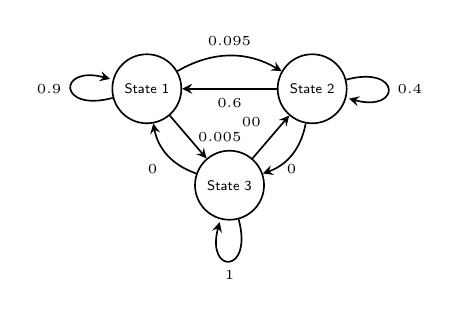
\begin{tikzpicture}[>=stealth, auto, node distance=4cm, semithick,scale=0.35]
        % Define styles for states
        \tikzstyle{state}=[circle, draw, minimum size=0.5cm, font=\sffamily\tiny]
    
        % Nodes with color fill
        \node[state] (Sunny) at (-3,1.5) {State 1};
        \node[state] (Cloudy) at (3,1.5) {State 2};
        \node[state] (Rainy) at (0,-2) {State 3};

    % Edges with arrows and transition probabilities
    \path
        (Sunny) edge [->, loop left] node {\tiny 0.9} ()
               edge [->, bend left] node {\tiny 0.095} (Cloudy)
               edge [->,right] node {\tiny 0.005} (Rainy)
        (Cloudy) edge [->, below] node {\tiny 0.6} (Sunny)
                edge [->, loop right] node {\tiny 0.4} ()
                edge [->, bend left] node [below] {\tiny 0} (Rainy)
        (Rainy) edge [->, bend left] node {\tiny 0} (Sunny)
               edge [->] node {\tiny 00} (Cloudy)
               edge [->, loop below] node {\tiny 1} ();
    \end{tikzpicture}

}
\end{example}

\vspace{4mm}

\cols{
    \begin{itemize}
        \item $P_{i,j}$ contains probability going to state $i$ from $j$
    \end{itemize}
}{
\onslide<2>{
$$P =
\left(%
\begin{array}{lll}
  .9 & .6 & 0 \\
  .095 & .4 & 0 \\
  .005 & 0 & 1 \\
\end{array}%
\right)
$$
}
}

\end{frame}

%%%%%%%%%%%%%%%%%%%%%%%%%%%%%%%%%%%%%%%%%%%%%%%%%%%%%%%%%%%%%%%%%%%%%%%%
\begin{frame}{Broken Machine Example}{Word Problem}

\begin{example}{Question}
If the machine is working on Day 1, what is the probability that it is still functional (that is, not permanently broken) a year from now?
\end{example}



   \begin{itemize}

      \item Take the 365'th power of the transition matrix:
         $$P^{365} =
         \left(%
         \begin{array}{lll}
           .9 & .6 & 0 \\
           .095 & .4 & 0 \\
           .005 & 0 & 1 \\
         \end{array}%
         \right)^{365} =
         \left(%
         \begin{array}{lll}
             0.1779 & 0.1792 & 0 \\
             0.0284 & 0.0286 & 0 \\
             \textcolor{red}{0.7937} & 0.7922 & 1
         \end{array}%
         \right)
         $$
    
    
    \item $P^{365}_{3,1} = 0.7937 \implies $ there's a 79.22\% chance that the machine is permanently broken after 365 days starting from state 1.  

    \begin{block}{Answer}
    If the machine is working on Day 1, it will not be permanently broken with probability of about 20.63\%. 
    \end{block}
   \end{itemize}
   
\end{frame}
%%%%%%%%%%%%%%%%%%%%%%%%%%%%%%%%%%%%%%%%%%%%%%%%%%%%%%%%%%%%%%%%%%%%%%%%%

\begin{frame}{Absorbing States}
\begin{itemize}

      \item This is the matrix one year from now
         $$P^{365} =
         \left(%
         \begin{array}{lll}
             0.1779 & 0.1792 & 0 \\
             0.0284 & 0.0286 & 0 \\
             \red{0.7937} & 0.7922 & 1
         \end{array}%
         \right)
         $$
          \item This is the matrix after two years 
         $$P^{365} =
         \left(%
         \begin{array}{lll}
             0.0367 & 0.0370 & 0 \\
             0.0059 & 0.0059 & 0 \\
             \red{0.9574} & 0.9571 & 1
         \end{array}%
         \right)
         $$
         \item As as the number of days $n\rightarrow \infty$, the odds of the printer being permanently broken approaches 1

         \define{Absorbing State}{
         A state $i$ in a Markov chain is an \textbf{absorbing state} if it has the transition probability $P_{ii}=1$
         }
\end{itemize}
\end{frame}

\begin{frame}{Absorbing States}
\begin{itemize}
      \item Suppose we begin with 
      $$x_0 = \begin{bmatrix}
          1\\0 \\0
      \end{bmatrix}$$

      \item As we iterate 
      $ x_n = P x_{n-1}$
      we eventually get 
      $$\lim_{n\rightarrow \infty} x_n = \begin{bmatrix}
          0\\0\\1
      \end{bmatrix}$$
    \item<2> This is connected to the \textit{power method}. The vector
    $$x=\begin{bmatrix}
        0\\0\\1
    \end{bmatrix}$$
    is the dominant eigenvalue of the matrix $P$, i.e. $Px = \lambda_1 x$
\end{itemize}
\end{frame}


%%%%%%%%%%%%%%%%%%%%%%%%%%%%%%%%%%%%%%%%%%%%%%%%%%%%%%%%%%%%%%
\sectionframe{Power Method and Markov Chains}
%%%%%%%%%%%%%%%%%%%%%%%%%%%%%%%%%%%%%%%%%%%%%%%%%%%%%%%%%%%%%%
\begin{frame}{Steady State Vector}

\begin{itemize}
    \item In many Markov chains, the state distribution stabilizes:
    \[
    x_{k+1} = Px_k \quad \longrightarrow \quad x_{k+1} \approx x_k
    \]
    \item When this happens, the system reaches a \textbf{steady state}

    \item A steady state vector $x$  must satisfy:
    \[
    Px = x
    \]
    which is the same as 
    $$
    Px = \lambda x
    $$
    where $\lambda=1$

    \define{Steady State}{
    \begin{itemize}
        \item  A steady state is an eigenvector of $P$ with eigenvalue $\lambda = 1$.
        \item When normalized, the steady state tells the long-term distribution of states.
    \end{itemize}
    }
\end{itemize}
\end{frame}


\begin{frame}{Connection to the Power Method}

\begin{itemize}
    \item Iterating a Markov chain means repeatedly computing:
    \[
    x_{k+1} = Px_k
    \]
    \item \emph{This is exactly the power method}
    \item The dominant eigenvector corresponds to steady state distribution of states in the Markov chain

    \item If $x_0$ is already normalized (sum of its elements is one) then you do \emph{not} have to normalize with each iteration
\end{itemize}

\keyidea{
If $P$ is the transition matrix for a Markov chain, then power method will give the steady state distribution of states.
}
\end{frame}


%%%%%%%%%%%%%%%%%%%%%%%%%%%%%%%%%%%%%%%%%%%%%%%%%%%%%%%%%%%%%%%%%%%%%%%%
\begin{frame}[fragile]{Weather Example}
\cols{\begin{center}
    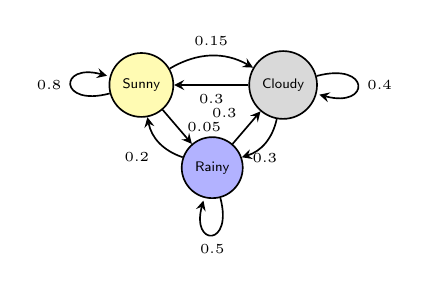
\begin{tikzpicture}[>=stealth, auto, node distance=3cm, semithick,scale=0.3]
        % Define styles for states
        \tikzstyle{state}=[circle, draw, minimum size=0.5cm, font=\sffamily\tiny]
    
        % Nodes with color fill
        \node[state, fill=yellow!30] (Sunny) at (-3,1.5) {Sunny};
        \node[state, fill=gray!30] (Cloudy) at (3,1.5) {Cloudy};
        \node[state, fill=blue!30] (Rainy) at (0,-2) {Rainy};

    % Edges with arrows and transition probabilities
    \path
        (Sunny) edge [->, loop left] node {\tiny 0.8} ()
               edge [->, bend left] node {\tiny 0.15} (Cloudy)
               edge [->,right] node {\tiny 0.05} (Rainy)
        (Cloudy) edge [->, below] node {\tiny 0.3} (Sunny)
                edge [->, loop right] node {\tiny 0.4} ()
                edge [->, bend left] node [below] {\tiny 0.3} (Rainy)
        (Rainy) edge [->, bend left] node {\tiny 0.2} (Sunny)
               edge [->] node {\tiny 0.3} (Cloudy)
               edge [->, loop below] node {\tiny 0.5} ();
    \end{tikzpicture}
    \end{center}
}{    
$$P =
\left(%
\begin{array}{lll}
  .8 & .3 & .2 \\
  .15 & .4 & .3 \\
  .05 & .3 & .5 \\
\end{array}%
\right)
$$
}
% \begin{lstlisting}[mathescape]
% >> [V, E] = eigs(P); 
% >> v1 = V(:,1); % get largest eigenvector
% >> v1 = v1/sum(v1) % scale eigenvector
% v1 =
%     0.5600
%     0.2400
%     0.2000
% \end{lstlisting}
% This tells us that around 56\% of the days are sunny. 

\begin{itemize}
    \item Start with $x_0=[1 \quad 0 \quad0]^T$ and iterate $x_{n+1} = Px_n$
    $$
    x_1=\begin{bmatrix}
        0.8\\0.15\\0
    \end{bmatrix},\quad
    x_2=\begin{bmatrix}
        0.695\\0.195\\0.11
    \end{bmatrix},\dots,\quad 
    x_{16}=\begin{bmatrix}
        0.56\\0.24\\0.20
    \end{bmatrix}
    $$
    \item $56\%$ days are sunny, $24\%$ days are cloudy, $20\%$ days are rainy
\end{itemize}

\end{frame}

%%%%%%%%%%%%%%%%%%%%%%%%%%%%%%%%%%

\begin{frame}{Exam Grade Example}
\cols{\begin{center}
    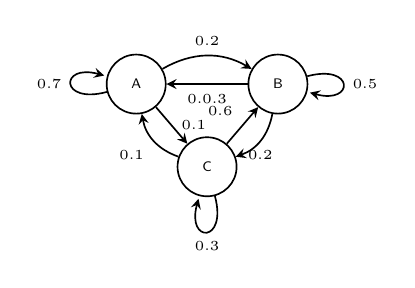
\begin{tikzpicture}[>=stealth, auto, node distance=3cm, semithick,scale=0.3]
        % Define styles for states
        \tikzstyle{state}=[circle, draw, minimum size=0.75cm, font=\sffamily\tiny]
    
        % Nodes with color fill
        \node[state] (A) at (-3,1.5) {A};
        \node[state] (B) at (3,1.5) {B};
        \node[state] (C) at (0,-2) {C};

    % Edges with arrows and transition probabilities
    \path
        (A) edge [->, loop left] node {\tiny 0.7} ()
               edge [->, bend left] node {\tiny 0.2} (B)
               edge [->,right] node {\tiny 0.1} (C)
        (B) edge [->, below] node {\tiny 0.0.3} (A)
                edge [->, loop right] node {\tiny 0.5} ()
                edge [->, bend left] node [below] {\tiny 0.2} (C)
        (C) edge [->, bend left] node {\tiny 0.1} (A)
               edge [->] node {\tiny 0.6} (B)
               edge [->, loop below] node {\tiny 0.3} ();
    \end{tikzpicture}
    \end{center}
}{    
$$P =
\left(%
\begin{array}{lll}
        0.7 & 0.3 & 0.1\\
        0.2 & 0.5 & 0.6\\
        0.1 & 0.2 & 0.3
\end{array}%
\right)
$$
}

\begin{itemize}
    \item Start with $x_0=[0.5 \quad 0 \quad0.5]^T$ and iterate $x_{n+1} = Px_n$
    $$
    x_1=\begin{bmatrix}
        0.4\\0.4\\0.2
    \end{bmatrix},\quad
    x_2=\begin{bmatrix}
        0.42\\0.40\\0.18
    \end{bmatrix},\dots,\quad 
    x_{10}=\begin{bmatrix}
        0.4423\\0.3846\\0.1731
    \end{bmatrix}
    $$
    \item If there were $\infty$ exams the final distribution will be
    $44\%$ A, $38\%$ B, and $17\%$ C 
\end{itemize}
    
\end{frame}

%%%%%%%%%%%%%%%%%%%%%%%%%%%%%%%%

\begin{frame}[fragile]{Broken Machine Example}

\begin{lstlisting}[mathescape]
>> P = [.9, .6, 0; .095, .4, 0; .005, 0, 1];
>> [V,E] = eigs(P)  
V =    
         0   -0.6496    0.7096 % columns are eigenvectors 
         0   -0.1036   -0.7045
    1.0000    0.7532   -0.0051

E =
    1.0000         0         0  %  eigenvalues
         0    0.9957         0
         0         0    0.3043

\end{lstlisting}

\keyidea{
\begin{itemize}
\item The largest eigenvalue is $\lambda=1$ and it has the eigenvector $v = [ 0\quad 0\quad 1]^T$
\item The vector $v = [ 0\quad 0\quad 1]^T$ is giving us the steady state \textit{probability distribution} of the states
\end{itemize}
}
\end{frame}

%%%%%%%%%%%%%%%%%%%%%%%%%%%%%%%%%%%%%%%%%%%%%%%%%%%%%%%%%%%%%%%%%%%%%
\sectionframe{Summary}
%%%%%%%%%%%%%%%%%%%%%%%%%%%%%%%%%%%%%%%%%%%%%%%%%%%%%%%%%%%%%%%%%%%%%

\begin{frame}{Markov Chains}
\begin{itemize}
    \item Suppose an object changes between states at discrete time steps
        $$X = \{\text{sunny}, \text{cloudy}, \text{rainy}\}$$
    \item Probability of jumping between states are known
    \begin{center}
    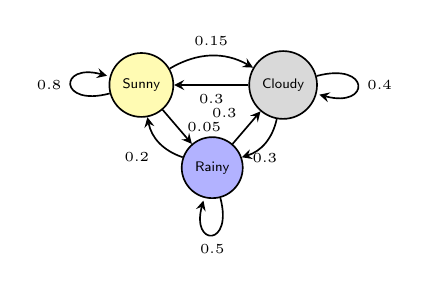
\begin{tikzpicture}[>=stealth, auto, node distance=3cm, semithick,scale=0.3]
        % Define styles for states
        \tikzstyle{state}=[circle, draw, minimum size=0.5cm, font=\sffamily\tiny]
    
        % Nodes with color fill
        \node[state, fill=yellow!30] (Sunny) at (-3,1.5) {Sunny};
        \node[state, fill=gray!30] (Cloudy) at (3,1.5) {Cloudy};
        \node[state, fill=blue!30] (Rainy) at (0,-2) {Rainy};

    % Edges with arrows and transition probabilities
    \path
        (Sunny) edge [->, loop left] node {\tiny 0.8} ()
               edge [->, bend left] node {\tiny 0.15} (Cloudy)
               edge [->,right] node {\tiny 0.05} (Rainy)
        (Cloudy) edge [->, below] node {\tiny 0.3} (Sunny)
                edge [->, loop right] node {\tiny 0.4} ()
                edge [->, bend left] node [below] {\tiny 0.3} (Rainy)
        (Rainy) edge [->, bend left] node {\tiny 0.2} (Sunny)
               edge [->] node {\tiny 0.3} (Cloudy)
               edge [->, loop below] node {\tiny 0.5} ();
    \end{tikzpicture}
    \end{center}
    \item System can be described with a \textit{transition matrix} $P$
\end{itemize}
\end{frame}

%%%%%%%%%%%%%%%%%%%%%%%%%%%%%%%%%%%%%%%%%%%%%%%%%%%%%%%%%%%%%%%%%%%%%%%%
\begin{frame}{Power Method}

    \begin{itemize}
        \item \textbf{Power Method} is a simple algorithm to find the \textit{dominant} eigenvector of a matrix
        \vfill 
        \item Doing the power method on the \textit{transition matrix} $P$ yields the \textit{steady-state distribution} of the system
    \end{itemize}
    
\end{frame}


%%%%%%%%%%%%%%%%%%%%%%%%%%%%%%%%%%%%%%%%%%%%%%%%%%%%%%%%%%%%%%%%%%%%%%%%
\sectionframe{Fun with Markov}
%%%%%%%%%%%%%%%%%%%%%%%%%%%%%%%%%%%%%%%%%%%%%%%%%%%%%%%%%%%%%%%%%%%%%%%%

\begin{frame}{Application: Text Prediction}

\begin{itemize}
    \item Many text models assume the next word depends only on the current word
    \item This is exactly a Markov chain assumption
\end{itemize}

\begin{example}
States = words in a vocabulary  
\[
P_{ij} = \Pr(\text{next word is } i \mid \text{current word is } j)
\]
\end{example}

\keyidea{
\begin{itemize}
    \item Markov chains model local structure, not global meaning.
    \item If something can be described as a locally dependent sequence, you can use \textit{Markov chains}
\end{itemize}
}
\end{frame}

\begin{frame}{Application: Text Prediction}
\textbf{Setup:}
\begin{enumerate}
    \item Choose a text
    \item List all unique words
    \item Count how often each word follows another word
    \item Normalize counts to form a transition matrix $P$
\end{enumerate}
\vfill
\textbf{Text Generation:}
\begin{enumerate}
    \item Pick a starting word
    \item Look up the corresponding probability column
    \item Randomly choose the next word using those probabilities
    \item Repeat
\end{enumerate}
    
\end{frame}

\begin{frame}{Application: Text Prediction}
\begin{example}
\textbf{Cat in the Hat} --- Dr. Seuss

\begin{verse}
The sun did not shine.\\
It was too wet to play.\\
So we sat in the house\\
All that cold, cold, wet day...
\end{verse}
\end{example}
\vfill

 \begin{block}{Generated Text}
 \ttfamily
    \begin{itemize}
        \item The cat in bed, Oh! What made for fish! 
        \item It stop you sir. Step this way. We fight these.
        \item The cat have come look. Then he said, "the box."
        \item It up the tags, it up the things, and he was gone with fear.
    \end{itemize}
 \end{block}
    
\end{frame}


%%%%%%%%%%%%%%%%%%

\begin{frame}{Application: Music Recommendation}

\begin{itemize}
    \item Spotify chooses what song to play next based on transition between music types
    \item The \textbf{states} are chosen to be categories:
    \begin{itemize}
        \item a genre (Rock, Pop, Jazz)
        \item an artist
        \item a song cluster (similar style or mood)
    \end{itemize}
    \item Each listen represents a transition from one state to another
\end{itemize}

\keyidea{
Assume that the song you want to listen to next depends on what you just finished listening to.
}
\end{frame}

%%%%%%%%%%%%%%%%%%%%%%%%%

\begin{frame}{How the Transition Matrix Is Built}

\begin{itemize}
    \item Music apps record user data:
    \[
    \text{Rock} \rightarrow \text{Rock} \rightarrow \text{Pop} \rightarrow \text{Jazz}
    \]
    \item Each transition is counted:
    \begin{itemize}
        \item Rock $\to$ Rock (120,000 times)
        \item Rock $\to$ Pop (30,000 times)
        \item Pop $\to$ Jazz (5,000 times)
    \end{itemize}
    \item These counts form a \textbf{transition count matrix}
\end{itemize}

\vspace{2mm}
\begin{block}{From Counts to Probabilities}
Each column is normalized so probabilities sum to 1.
\end{block}

\end{frame}

%%%%%%%%%%%%%

\begin{frame}{Example}

Let the states be music genres:
\[
\{\text{Rock},\ \text{Indie},\ \text{Pop},\ \text{Hip-Hop},\ \text{Jazz}\}
\]

\vspace{2mm}
We define the transition probabilities
\[
P_{ij} = \Pr(\text{next song is genre } i \mid \text{current song is genre } j)
\]

\begin{itemize}
    \item Columns represent the \textbf{current genre}
    \item Rows represent the \textbf{next genre}
    \item Each column sums to 1
\end{itemize}

\vspace{3mm}
\textbf{Example (illustrative numbers):}

\[
P =
\begin{bmatrix}
0.60 & 0.20 & 0.10 & 0.10 & 0.30 \\
0.20 & 0.50 & 0.20 & 0.10 & 0.20 \\
0.10 & 0.20 & 0.50 & 0.30 & 0.10 \\
0.05 & 0.05 & 0.15 & 0.40 & 0.05 \\
0.05 & 0.05 & 0.05 & 0.10 & 0.35
\end{bmatrix}
\]

\end{frame}



%%%%%%%%%%%%%%%%%%%%%%%%%%%%%%%%%%%%%%%%%%%%%%%%%%%%%%%%%%%%%%%%%%%%%%%%
% \sectionframe{Google Pagerank}
% %%%%%%%%%%%%%%%%%%%%%%%%%%%%%%%%%%%%%%%%%%%%%%%%%%%%%%%%%%%%%%%%%%%%%%%%

\begin{frame}{Web Pages}

\begin{figure}
    \centering
    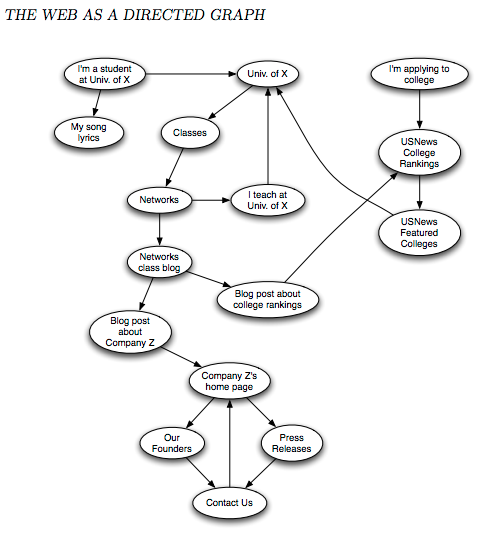
\includegraphics[width=0.5\linewidth]{figs/Web_directed_graph.png}
    \caption{Web pages can be turned into a matrix.}
\end{figure}

\end{frame}

% %%%%%%%%%%%%%%%%%%%%%%%%%%%%%%%%%%%%%%%%%%%%%%%%%%%%%%%%%%%%%%%%%%%%%%%%%
\begin{frame}{Google PageRank}
    \begin{block}{Web Structure}
        \begin{itemize}
            \item Let $W$ be the set of web pages that can be reached by following a chain of hyperlinks starting from a page on Google.
            \item Let $n$ be the number of pages in $W$.
        \end{itemize}
    \end{block}
    
    \vspace{2mm}
    
    \begin{block}{Connectivity and Transition Matrices}
        \begin{itemize}
            \item Let $G$ be the $n \times n$ \textbf{connectivity matrix} of $W$, where
            \[
            G_{i,j} = 
            \begin{cases}
                1 & \text{if there is a hyperlink from page } j \text{ to page } i, \\
                0 & \text{otherwise}.
            \end{cases}
            \]
            \item Rescale the \textbf{transition matrix} $G$ by normalizing each column of $G$ by the number of outgoing links from page $j$:
            \[
            G_{i,j} = \frac{G_{i,j}}{\text{outdegree}(j)}
            \]
        \end{itemize}
    \end{block}
\end{frame}
%%%%%%%%%%%%%%%%%%%%%%%%%%%%%%%%%%%%%%%%%%%%%%%%%%%%%%%%%%%%%%%%%%%%
\begin{frame}{How Google Search Works}

\begin{enumerate}
    \item Find a list of $n$ websites containing keywords
    \item Generate a directed graph from the webpages 
    \item Generate a transition matrix $P$
    \item Do power method on $P$
    \item Sort the dominant eigenvector from greatest to least 
    \item Display websites corresponding to sorted eigenvector
\end{enumerate}

\textbf{Result}: A list of websites ordered in terms of relevancy
\end{frame}

%%%%%%%%%%%%%%%%%%%%%%%%%%%%%%%%%%%%%%%%%%%%%%%%%%%%%%%%%%%%%%%%%%%%

% \begin{frame}{The Random Walk}
% Google made a simple model of a random web surfer:
% \begin{enumerate}
%     \item Start at any webpage 
%     \item Randomly click a link on the page 
%     \item Repeat
% \end{enumerate}

%     \vspace{6mm}

% Outcomes of the Random Walk:
% \begin{itemize}
%     \item \textbf{Dead End}: Find pages with no external links
%     \item \textbf{Cycle}: Find series of pages that form an infinite cycle
%     \item \textbf{Limiting Probability}: Find pages that have a high frequency of visits 
% \end{itemize}
% \end{frame}
%%%%%%%%%%%%%%%%%%%%%%%%%%%%%%%%%%%%%%%%%%%%%%%%%%%%%%%%%%%%%%%%%%%%%%%%

% \begin{frame}{Google and Probability}
%     \begin{itemize}
%         \item Let $c_j$ and $r_i$ be the column and row sums of $G$, respectively:
%         \[
%         c_j = \sum_{i} G_{i,j}, \quad r_i = \sum_{j} G_{i,j}
%         \]
        
%         \item Then:
%         \begin{itemize}
%             \item $r_k$ is the \textbf{indegree} of page $k$ (number of links into page $k$).
%             \item $c_k$ is the \textbf{outdegree} of page $k$ (number of outgoing links from page $k$).
%         \end{itemize}
%         \bigskip
        
%         \item Let $p$ be the fraction of time that the random walk follows a specific hyperlink.
%         \item Google typically sets $p = 0.85$.
%         \item Consequently, $1-p$ represents the fraction of time that the random walker jumps to a random page.
%     \end{itemize}
% \end{frame}

%%%%%%%%%%%%%%%%%%%%%%%%%%%%%%%%%%%%%%%%%%%%%%%%%%%%%%%%%%%%%%%%%%%%%%%%%

% \begin{frame}{Google meets Markov}
% \begin{itemize}
% \item Let $A$ be an $n \times n$ matrix whose elements are
% \[A_{i,j}
% = \begin{cases}p\, G_{i,j}/c_j + \delta, \quad &c_j \neq 0 \\
% 1/n, \quad  &c_j = 0
% \end{cases}
% \]
%  where $\delta = (1-p)/n$.
% \item This matrix is the transition matrix of the Markov chain of
% a random walk!
% \item Notice that $A$ comes from scaling the connectivity matrix
% by its column sums.
% \item The $j$-th column is the probability of jumping from the
% $j$-th page to the other pages on the Web.
% \end{itemize}
% \end{frame}
%%%%%%%%%%%%%%%%%%%%%%%%%%%%%%%%%%%%%%%%%%%%%%%%%%%%%%%%%%%%%%%%%%%%%%%%%


%%%%%%%%%%%%%%%%%%%%%%%%%%%%%%%%%%%%%%%%%%%%%%%%%%%%%%%%%%%%%%%%%%%%%%%%%
%\begin{frame}
%    \frametitle{The problem}
%Can write $A$, the transition matrix, as
%\[
%A = p G D + e z^T
%\]
%where $e$ is the vector of all ones and where $ez^T$ account for dead linked 
%pages and 
%\[
%D_{jj} = 1/c_j \,\textnormal{(or 0)}\quad z_j = \delta\, \textnormal{(or $1/n$)}
%\]
%Then $x=Ax$ can be written
%\[
% (I-pGD)x = (z^Tx) e = \gamma e
%\]
%and we can scale $x$ such that $\gamma=1$
%
%see \texttt{pagerank.m}
%\end{frame}
%%%%%%%%%%%%%%%%%%%%%%%%%%%%%%%%%%%%%%%%%%%%%%%%%%%%%%%%%%%%%%%%%%%%%%%%
% \begin{frame}{Eigenvectors and Google}

% Find $x = Ax$ and the elements of $x$ are Google's PageRank.
%    \begin{itemize}
      
%       \item That is, $x$ is the result of an infinite walk 
%          $$x \leftarrow A*A*\dots*A v$$ 
%          for any starting vector $v$.
      
%       \item And element $i$ of $x$ (i.e., $x_i$) is the probability that you
%          ended up on page $i$
      
%       \item As implied by the earlier example of an office machine, this $x$ is
%          the eigenvector of largest eigenvalue, and the eigenvalue is $1$ \newline
%          $\Rightarrow$ Use the power method!

%    \end{itemize}

% \bigskip
% \bigskip

% For any particular search string, 
% \begin{itemize}
%    \item First, Google finds pages on the Web that match the search string
%    \item Second, the pages are listed in the order of their PageRank.
% \end{itemize}
% \end{frame}
%%%%%%%%%%%%%%%%%%%%%%%%%%%%%%%%%%%%%%%%%%%%%%%%%%%%%%%%%%%%%%%%%%%%%%%%%
%%%%%%%%%%%%%%%%%%%%%%%%%%%%%%%%%%%%%%%%%%%%%%%%%%%%%%%%%%%%%%%%%%%%%%%%
% \begin{frame}
% \frametitle{Matlab}
% \framesubtitle{Moler's scripts}

% \begin{itemize}
%    \item To search from a homepage, you will type a statement like:
%    \bigskip

%    \texttt{[U,G] = surfer('http://www.unm.edu',n)}
%    \bigskip

%    \item This starts at the given URL and tries to surf the Web until it
%    has visited $n$ pages.  That is, an $n$ by $n$ matrix is formed.
%    \bigskip

%    \item Note, \texttt{surfer.m} is very primitive...
%    %\bigskip

%    %\item Try, \texttt{[U, G] = surfer('http://www.unm.edu', 5)}\\
%    %   and inspect \texttt{U, G}

% \end{itemize}
% \end{frame}
% %%%%%%%%%%%%%%%%%%%%%%%%%%%%%%%%%%%%%%%%%%%%%%%%%%%%%%%%%%%%%%%%%%%%%%%%%
% %%%%%%%%%%%%%%%%%%%%%%%%%%%%%%%%%%%%%%%%%%%%%%%%%%%%%%%%%%%%%%%%%%%%%%%%
% \begin{frame}
% \frametitle{Matlab}
% \framesubtitle{Moler's scripts}
% \begin{itemize}
%   \item Download \texttt{surfer.m}, \texttt{pagerank.m} and \texttt{pagerankpow.m}

%   \item \texttt{[U,G] = surfer('http://www.unm.edu',20);}
%   \begin{description}
%     \item[$U$] = a cell array of $n$ strings, the URLs of the nodes.
%     \item[$G$]= an $n$-by-$n$ sparse matrix with $G(i,j)=1$ if node $j$
%     is linked to node $i$.
%   \end{description}
%   \item Next: \texttt{spy(G)}.  This shows the nonzero
% structure of the connectivity matrix.
%   \item Finally: \texttt{pagerank(U,G)} and the pagerank will
%      be computed for all 20 pages (see generated bar chart)
% \end{itemize}
% \end{frame}
%%%%%%%%%%%%%%%%%%%%%%%%%%%%%%%%%%%%%%%%%%%%%%%%%%%%%%%%%%%%%%%%%%%%%%%%%

%%%%%%%%%%%%%%%%%%%%%%%%%%%%%%%%%%%%%%%%%%%%%%%%%%%%%%%%%%%%%%%%%%%%%%%%%
% \begin{frame}{Summary}

% How PageRanks works:
% \vspace{4mm}
% \begin{enumerate}
%     \item Form transition matrix $A$ from Google matrix $G$.\\[4mm]  
    
%     \item Estimate the largest eigenvector of $A$ with \underline{power method}.\\[4mm]

%     \item Normalize then sort the elements of the eigenvector.\\[4mm]
   
%     \item Return list of website in order according to sort index. 
% \end{enumerate}    
% \end{frame}
%%%%%%%%%%%%%%%%%%%%%%%%%%%%%%%%%%%%%%%%%%%
\end{document}
